\section[Architetture non Von Neumann]{Architetture non Von Neumann}
\label{sec:pipeline}
\sectionframe{images/covers/cover_pipeline.png}{Architetture \protect\linebreak non Von Neumann}	 
 

\begin{frame}
	\frametitle{Aumentare le prestazioni delle CPU}

	\begin{block}{Aumentare le prestazioni delle CPU}
		Per potenziare le prestazioni delle CPU e dei sistemi di elaborazione, rimanendo ancorati ad una architettura di Von Neumann, sono state prese in considerazione diverse strategie:
		\begin{itemize}
			\item l'incremento della frequenza di clock
			\item l'ampliamento della dimensione della parola
			\item l'aumento dello spazio di indirizzamento
		\end{itemize}
		
		Tuttavia, tutte queste strategie hanno raggiunto un punto limite nell'evoluzione delle architetture, oltre il quale ulteriori miglioramenti delle prestazioni sono diventati sempre più difficili.\\~\\
		
		Di conseguenza, è emersa un'altra prospettiva di sviluppo attraverso l'approccio di \textbf{architetture non Von Neumann}.
	\end{block}

\end{frame}


\begin{frame}
	\frametitle{Aumentare le prestazioni delle CPU}

	\begin{figure}[!htbp]
		\centering
		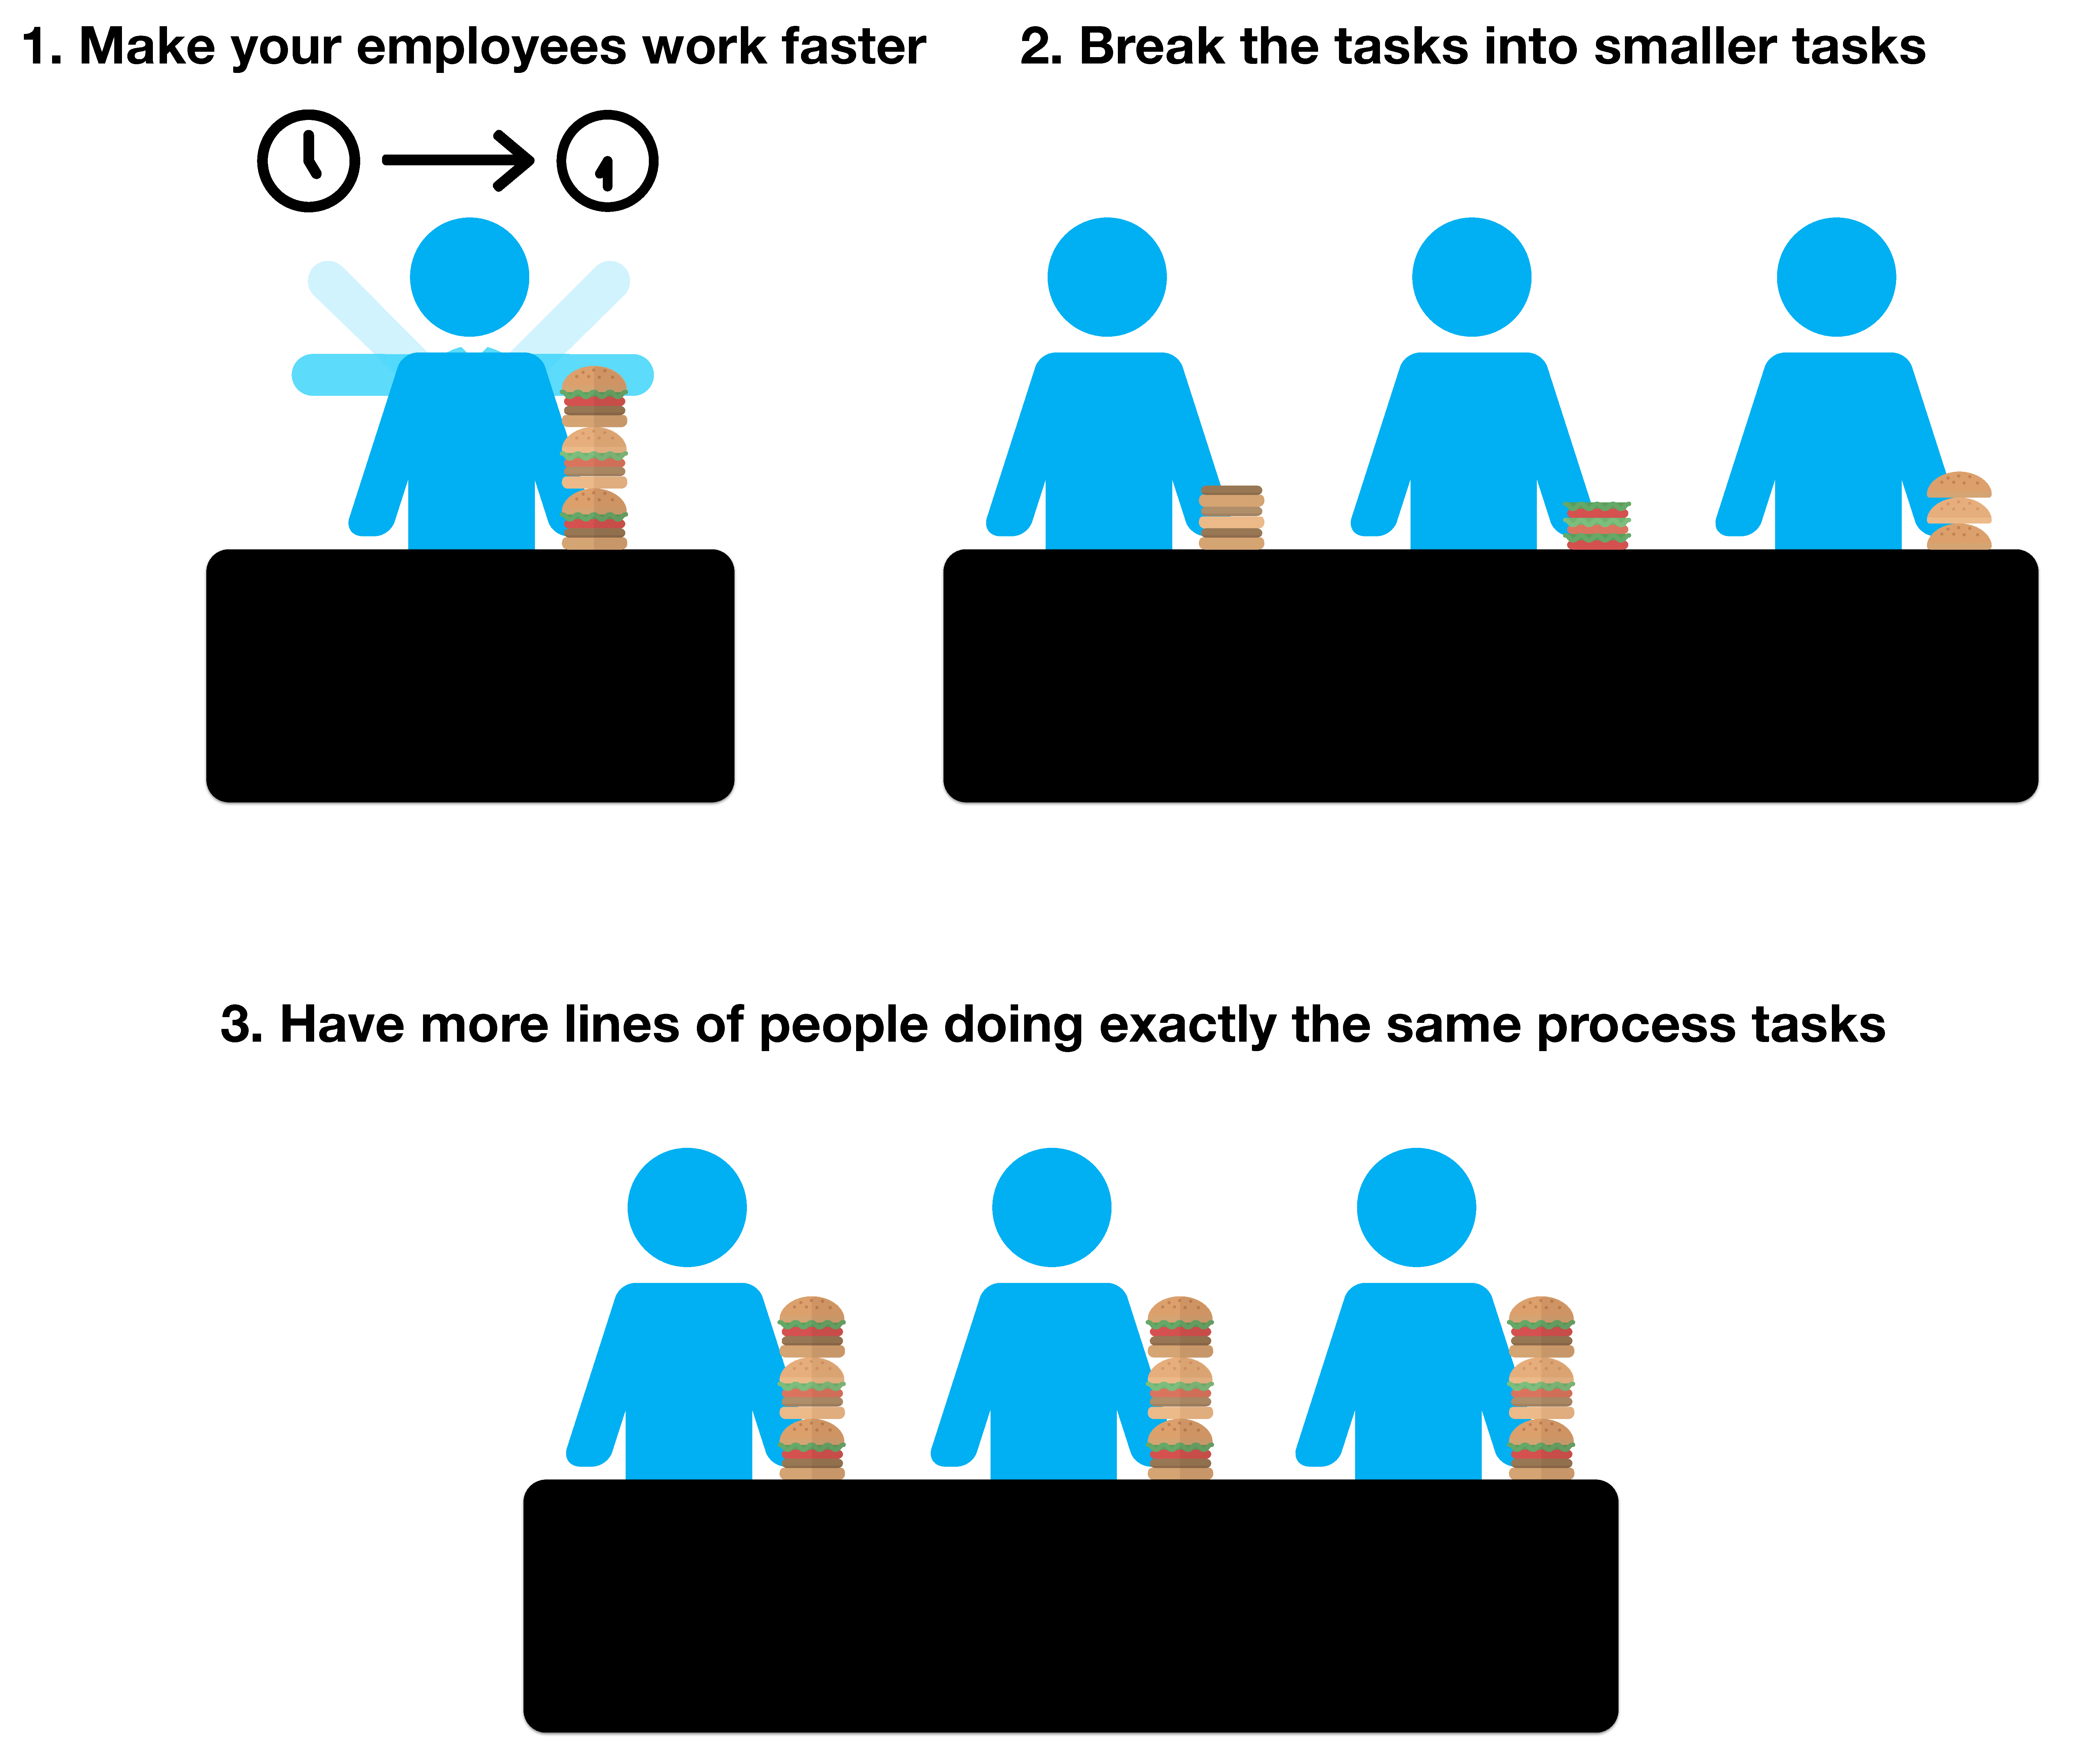
\includegraphics[width=0.73\linewidth]{images/7_pipeline/faster_cpu.pdf}
		%\caption{}
%		\label{}
	\end{figure}
\end{frame}


\begin{frame}
	\frametitle{Architetture non Von Neumann}

	\begin{block}{Architetture non Von Neumann}
		Elenchiamo alcune di questi possibili approcci:
		\begin{enumerate}
			\item Esecuzione fuori ordine
			\item Prefetch
			\item Speculative execution
			\item Pipeline
			\item Branch prediction
			\item Cache memory
			\item DMA (Direct Memory Access)
			\item Coprocessori
		\end{enumerate}
	\end{block}

\end{frame}


\subsection[Esecuzione fuori ordine]{Esecuzione fuori ordine}
\begin{frame}
	\frametitle{\textbullet{1} Esecuzione fuori ordine}

	%\begin{block}{Esecuzione fuori ordine}
		L'esecuzione fuori ordine è una tecnica avanzata utilizzata nelle CPU per migliorare l'efficienza nell'esecuzione delle istruzioni. Invece di eseguire le istruzioni nell'ordine in cui sono state ricevute, come accadeva nelle prime architetture, l'esecuzione fuori ordine permette alla CPU di eseguire istruzioni indipendenti in parallelo, sfruttando al massimo le risorse disponibili.\vspace{0.5em}
		
		Quando una CPU opera in modalità di esecuzione fuori ordine, può analizzare le istruzioni in entrata e identificare quelle che possono essere eseguite senza dipendenze da istruzioni precedenti. Queste istruzioni vengono inviate alle unità di esecuzione in parallelo, indipendentemente dall'ordine originale. Questo metodo non sempre può essere impiegato. Qualora due istruzioni consecutive siano dipendenti (ad esempio se la seconda istruzione usa il risultato ottenuto dalla prima istruzione) è necessario rispettare la sequenza operativa e le due istruzioni non potranno essere eseguite in parallelo.
	%\end{block}

\end{frame}


\begin{frame}
	\frametitle{\textbullet{1} Esecuzione fuori ordine}

	%\begin{block}{Esecuzione fuori ordine}
		L'esecuzione fuori ordine richiede hardware complesso, come buffer per riordinare i risultati in base all'ordine originale, unità di predizione delle dipendenze e logica per garantire l'integrità delle operazioni. Questa tecnica ha dimostrato di migliorare notevolmente le prestazioni delle CPU, consentendo loro di eseguire più istruzioni in modo parallelo e ottimizzato, pur mantenendo l'ordine corretto dei risultati in uscita.% \\~\\
		
		%
		
		\begin{figure}[!htbp]
			\centering 
			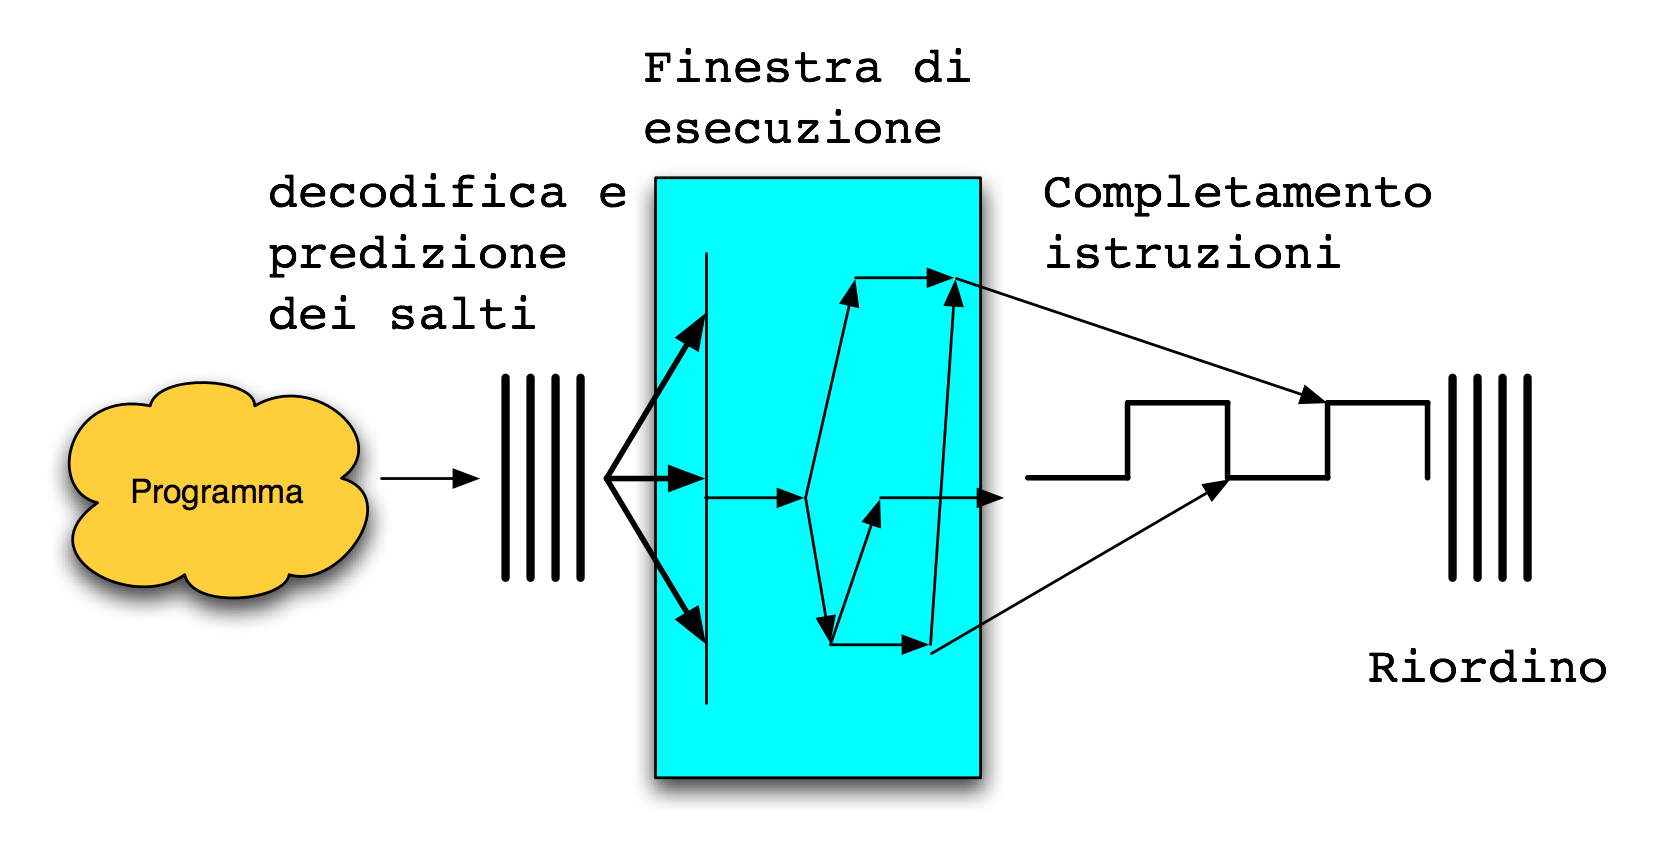
\includegraphics[width=0.7\linewidth]{images/7_pipeline/superscalar_processor.png}
			%\caption{}
			\label{fig:pipeline_superscalar_processor}
		\end{figure}
	%\end{block}

\end{frame}



\subsection[Prefetch]{Prefetch}
\subsection[Speculative execution]{Speculative execution}
\subsection[Pipeline]{Pipeline}
\subsection[Branch prediction]{Branch prediction}
\subsection[Cache memory]{Cache memory}
\subsection[DMA (Direct Memory Access)]{DMA (Direct Memory Access)}
\subsection[Coprocessori]{Coprocessori}





%\subsection[Central Processing Unit]{Central Processing Unit}
%\begin{frame}
%	\frametitle{Central Processing Unit}
%	
%%	\begin{block}{Central Processing Unit}
%		Una CPU, \textbf{central processing unit} (unità centrale di elaborazione o processore centrale), indica un'unità o sottosistema logico e fisico che sovraintende alle \textbf{funzionalità logiche di elaborazione} principali di un computer.
%		La CPU è un'elaborata combinazione di transistor che può essere definita \textit{circuito integrato}.\\~\\
%		\pause
%		All'interno della CPU individuiamo tre elementi fondamentali:
%		\begin{itemize}
%			\item \textbf{la CU}, \textit{Control Unit} (l’unità di controllo):\\
%			coordina l'esecuzione delle operazioni da parte del processore;
%			\item \textbf{la ALU}, \textit{Arithmetic-Logic Unit} (l’Unità Aritmetico-Logica):\\
%			si occupa di eseguire le operazioni aritmetico-logiche;
%			\item \textbf{i registri di memoria}:\\
%			diverse \textit{celle di memoria} dedicate a scopi specifici che vengono utilizzati per il controllo dell'esecuzione di un programma.
%		\end{itemize}
%%	\end{block}
%	
%\end{frame}


